\documentclass{sigchi}

% Use this command to override the default ACM copyright statement (e.g. for preprints). 
% Consult the conference website for the camera-ready copyright statement.


%% EXAMPLE BEGIN -- HOW TO OVERRIDE THE DEFAULT COPYRIGHT STRIP -- (July 22, 2013 - Paul Baumann)
% \toappear{Permission to make digital or hard copies of all or part of this work for personal or classroom use is 	granted without fee provided that copies are not made or distributed for profit or commercial advantage and that copies bear this notice and the full citation on the first page. Copyrights for components of this work owned by others than ACM must be honored. Abstracting with credit is permitted. To copy otherwise, or republish, to post on servers or to redistribute to lists, requires prior specific permission and/or a fee. Request permissions from permissions@acm.org. \\
% {\emph{CHI'14}}, April 26--May 1, 2014, Toronto, Canada. \\
% Copyright \copyright~2014 ACM ISBN/14/04...\$15.00. \\
% DOI string from ACM form confirmation}
%% EXAMPLE END -- HOW TO OVERRIDE THE DEFAULT COPYRIGHT STRIP -- (July 22, 2013 - Paul Baumann)


% Arabic page numbers for submission. 
% Remove this line to eliminate page numbers for the camera ready copy
% \pagenumbering{arabic}


% Load basic packages
\usepackage{balance}  % to better equalize the last page
\usepackage{graphics} % for EPS, load graphicx instead
\usepackage{times}    % comment if you want LaTeX's default font
\usepackage{url}      % llt: nicely formatted URLs

% llt: Define a global style for URLs, rather that the default one
\makeatletter
\def\url@leostyle{%
  \@ifundefined{selectfont}{\def\UrlFont{\sf}}{\def\UrlFont{\small\bf\ttfamily}}}
\makeatother
\urlstyle{leo}


% To make various LaTeX processors do the right thing with page size.
\def\pprw{8.5in}
\def\pprh{11in}
\special{papersize=\pprw,\pprh}
\setlength{\paperwidth}{\pprw}
\setlength{\paperheight}{\pprh}
\setlength{\pdfpagewidth}{\pprw}
\setlength{\pdfpageheight}{\pprh}

% Make sure hyperref comes last of your loaded packages, 
% to give it a fighting chance of not being over-written, 
% since its job is to redefine many LaTeX commands.
\usepackage[pdftex]{hyperref}
\hypersetup{
pdftitle={SIGCHI Conference Proceedings Format},
pdfauthor={LaTeX},
pdfkeywords={SIGCHI, proceedings, archival format},
bookmarksnumbered,
pdfstartview={FitH},
colorlinks,
citecolor=black,
filecolor=black,
linkcolor=black,
urlcolor=black,
breaklinks=true,
}

% create a shortcut to typeset table headings
\newcommand\tabhead[1]{\small\textbf{#1}}


% End of preamble. Here it comes the document.
\begin{document}

\title{SIGCHI Conference Proceedings Format}

\numberofauthors{3}
\author{
  \alignauthor 1st Author Name\\
    \affaddr{Affiliation}\\
    \affaddr{Address}\\
    \email{e-mail address}\\
    \affaddr{Optional phone number}
  \alignauthor 2nd Author Name\\
    \affaddr{Affiliation}\\
    \affaddr{Address}\\
    \email{e-mail address}\\
    \affaddr{Optional phone number}    
  \alignauthor 3rd Author Name\\
    \affaddr{Affiliation}\\
    \affaddr{Address}\\
    \email{e-mail address}\\
    \affaddr{Optional phone number}
}

\maketitle

\begin{abstract}
In this paper we describe the formatting requirements for
SIGCHI Conference Proceedings, and this sample file
offers recommendations on writing for the worldwide
SIGCHI readership. Please review this document even if
you have submitted to SIGCHI conferences before, some
format details have changed relative to previous years.
\end{abstract}

\keywords{
	Guides; instructions; author's kit; conference publications;
	keywords should be separated by a semi-colon. \newline
	\textcolor{red}{Optional section to be included in your final version, 
  but strongly encouraged.}
}

\category{H.5.m.}{Information Interfaces and Presentation (e.g. HCI)}{Miscellaneous}

See: \url{http://www.acm.org/about/class/1998/}
for more information and the full list of ACM classifiers
and descriptors. \newline
\textcolor{red}{Optional section to be included in your final version, 
but strongly encouraged. On the submission page only the classifiers’ 
letter-number combination will need to be entered.}

\section{Introduction}

This format is to be used for submissions that are
published in the conference proceedings.  We wish to give
this volume a consistent, high-quality appearance. We
therefore ask that authors follow some simple\cite{Mather2000}
guidelines. In essence, you should format your paper
exactly like this document. The easiest way to do this is
simply to download a template from the conference web
site, and replace the content with your own material.

\section{Methodology}
\section{Findings}

\subsection{Manipulation Check}
We conducted a manipulation check to verify the success manipulation of our condition. After watching each video clip, we ask participants to rate the severity for each scenario. We found in all scenarios, the participants rated the severe condition significantly higher than the non-severe condition.

\begin{table}
  \centering
  \begin{tabular}{|c|c|c|c|}
    \hline
    Type & Non-Severe & Severe & p Value \\
    \hline
    Financial & 3.633 & 4.918 & 0.0003 \\
    \hline
    Psychological & 2.633 & 5.020 & $ < 0.0001$ \\
    \hline
    Psychological & 2.816 & 5.020 & $ < 0.0001$ \\
    \hline
  \end{tabular}
  \caption{Mean Difference between perceive severity}
  \label{tab:table1}
\end{table}

\subsection{Result}
To test our hypothesis, we carried analysis of variance (ANOVA) on the collected result. 

In our first hypothesis, we hypothesize that robots will be blamed significantly more than other stakeholders in the psychological harm condition. To verify the hypothesis we ran a one-way ANOVA on the result and found no evidence to support our hypothesize. We found participants blamed programmer the most(mean = 6.28) compare to other stakeholders. In relation to our hypothesis, participants blamed programmers($ F(1,582) =139.1, p < .0001$), owner ($ F(1,582) = 19.68, p < .0001$), manufacturer($F(1,582) = 38.28, p < .0001$) and manager($F(1,582) = 13.38, p = 0.0003$) more than the robot. Only customers were blamed significantly less than the robot($F(1,582) = 54.09, p < .0001$)

\begin{table}[h]
  \centering
  \begin{tabular}{|c|c|c|}
    \hline
    Stakeholders & Mean & Standard Deviation\\
    \hline
    Robot & 3.184 & 0\\
    \hline
    Customer & 1.255 & 0\\
    \hline
    Manager & 4.142 & 0 \\
    \hline
    Manufacturer & 4.806 & 0 \\
    \hline
    Owner & 4.34694 & 0 \\
    \hline
    Programmer & 6.286 & 0 \\
    \hline
  \end{tabular}
  \caption{Mean Difference between perceive severity}
  \label{tab:table2}
\end{table}



\section{Discussion}
\section{Conclusion}

%
%\begin{figure}[!h]
%\centering
%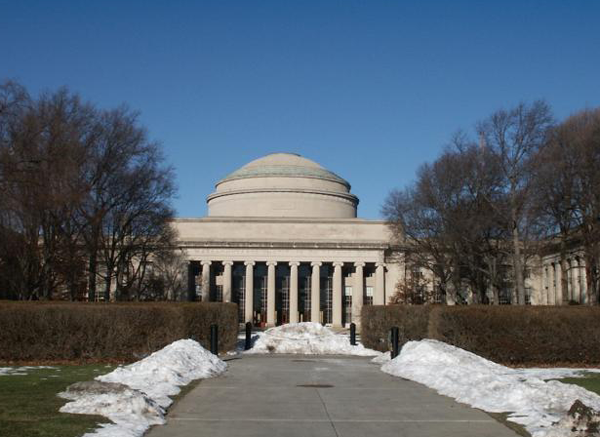
\includegraphics[width=0.9\columnwidth]{Figure1}
%caption{With Caption Below, be sure to have a good resolution image
%  (see item D within the preparation instructions).}
%\label{fig:figure1}
%\end{figure}
%


\section{References format}
References must be the same font size as other body text.
% REFERENCES FORMAT
% References must be the same font size as other body text.
\bibliographystyle{acm-sigchi}
\bibliography{reference}
\end{document}
